\documentclass[a4paper,11pt]{book}
%\documentclass[a4paper,twoside,11pt,titlepage]{book}
\usepackage{listings}
\usepackage[utf8]{inputenc}
\usepackage[spanish]{babel}

% \usepackage[style=list, number=none]{glossary} %
%\usepackage{titlesec}
%\usepackage{pailatino}

\decimalpoint
\usepackage{dcolumn}
\newcolumntype{.}{D{.}{\esperiod}{-1}}
\makeatletter
\addto\shorthandsspanish{\let\esperiod\es@period@code}
\makeatother


%\usepackage[chapter]{algorithm}
\RequirePackage{verbatim}
%\RequirePackage[Glenn]{fncychap}
\usepackage{fancyhdr}
\usepackage{graphicx}
\usepackage{afterpage}

\usepackage{longtable}

\usepackage[pdfborder={000}]{hyperref} %referencia

% ********************************************************************
% Re-usable information
% ********************************************************************
\newcommand{\myTitle}{TradingAPP}
\newcommand{\mySubtitle}{Aplicación web para trading algorítmico}
\newcommand{\mySubtitleEnglish}{Algorithmic trading web application}
\newcommand{\myDegree}{Grado en ingeniería informática}
\newcommand{\myName}{Manuel Carmona Pérez}
\newcommand{\myProf}{José Manuel Benítez Sánchez}
%\newcommand{\mySupervisor}{Put name here}
\newcommand{\myFaculty}{Escuela Técnica Superior de Ingenierías Informática y de
Telecomunicación}
\newcommand{\myFacultyShort}{E.T.S. de Ingenierías Informática y de
Telecomunicación}
\newcommand{\myDepartment}{Departamento de ...}
\newcommand{\myUni}{\protect{Universidad de Granada}}
\newcommand{\myLocation}{Granada}
\newcommand{\myTime}{\today}
\newcommand{\myVersion}{Version 0.1}


\hypersetup{
pdfauthor = {\myName (email (en) ugr (punto) es)},
pdftitle = {\myTitle},
pdfsubject = {},
pdfkeywords = {palabra_clave1, palabra_clave2, palabra_clave3, ...},
pdfcreator = {LaTeX con el paquete ....},
pdfproducer = {pdflatex}
}

%\hyphenation{}


%\usepackage{doxygen/doxygen}
%\usepackage{pdfpages}
\usepackage{url}
\usepackage{colortbl,longtable}
\usepackage[stable]{footmisc}
\usepackage{index}

\makeindex
%\usepackage[style=long, cols=2,border=plain,toc=true,number=none]{glossary}
% \makeglossary

% Definición de comandos que me son tiles:
%\renewcommand{\indexname}{Índice alfabético}
%\renewcommand{\glossaryname}{Glosario}

\pagestyle{fancy}
\fancyhf{}
\fancyhead[LO]{\leftmark}
\fancyhead[RE]{\rightmark}
\fancyhead[RO,LE]{\textbf{\thepage}}
\renewcommand{\chaptermark}[1]{\markboth{\textbf{#1}}{}}
\renewcommand{\sectionmark}[1]{\markright{\textbf{\thesection. #1}}}

\setlength{\headheight}{1.5\headheight}

\newcommand{\HRule}{\rule{\linewidth}{0.5mm}}
%Definimos los tipos teorema, ejemplo y definición podremos usar estos tipos
%simplemente poniendo \begin{teorema} \end{teorema} ...
\newtheorem{teorema}{Teorema}[chapter]
\newtheorem{ejemplo}{Ejemplo}[chapter]
\newtheorem{definicion}{Definición}[chapter]

\definecolor{gray97}{gray}{.97}
\definecolor{gray75}{gray}{.75}
\definecolor{gray45}{gray}{.45}
\definecolor{gray30}{gray}{.94}

\lstset{ frame=Ltb,
     framerule=0.5pt,
     aboveskip=0.5cm,
     framextopmargin=3pt,
     framexbottommargin=3pt,
     framexleftmargin=0.1cm,
     framesep=0pt,
     rulesep=.4pt,
     backgroundcolor=\color{gray97},
     rulesepcolor=\color{black},
     %
     stringstyle=\ttfamily,
     showstringspaces = false,
     basicstyle=\scriptsize\ttfamily,
     commentstyle=\color{gray45},
     keywordstyle=\bfseries,
     %
     numbers=left,
     numbersep=6pt,
     numberstyle=\tiny,
     numberfirstline = false,
     breaklines=true,
   }
 
% minimizar fragmentado de listados
\lstnewenvironment{listing}[1][]
   {\lstset{#1}\pagebreak[0]}{\pagebreak[0]}

\lstdefinestyle{CodigoC}
   {
	basicstyle=\scriptsize,
	frame=single,
	language=C,
	numbers=left
   }
\lstdefinestyle{CodigoC++}
   {
	basicstyle=\small,
	frame=single,
	backgroundcolor=\color{gray30},
	language=C++,
	numbers=left
   }

 
\lstdefinestyle{Consola}
   {basicstyle=\scriptsize\bf\ttfamily,
    backgroundcolor=\color{gray30},
    frame=single,
    numbers=none
   }


\newcommand{\bigrule}{\titlerule[0.5mm]}


%Para conseguir que en las páginas en blanco no ponga cabecerass
\makeatletter
\def\clearpage{%
  \ifvmode
    \ifnum \@dbltopnum =\m@ne
      \ifdim \pagetotal <\topskip
        \hbox{}
      \fi
    \fi
  \fi
  \newpage
  \thispagestyle{empty}
  \write\m@ne{}
  \vbox{}
  \penalty -\@Mi
}
\makeatother

\usepackage{pdfpages}
\begin{document}
\begin{titlepage}
 
 
\newlength{\centeroffset}
\setlength{\centeroffset}{-0.5\oddsidemargin}
\addtolength{\centeroffset}{0.5\evensidemargin}
\thispagestyle{empty}

\noindent\hspace*{\centeroffset}\begin{minipage}{\textwidth}

\centering

\includegraphics[width=0.9\textwidth]{imagenes/logo_ugr.jpg}\\[1.4cm]

\textsc{ \Large TRABAJO FIN DE GRADO\\[0.2cm]}
\textsc{ INGENIERÍA INFORMÁTICA }\\[1cm]
% Upper part of the page
% 
% Title
{\Huge\bfseries \myTitle \\}
\noindent\rule[-1ex]{\textwidth}{3pt}\\[3.5ex]
{\large\bfseries \mySubtitle \\}
\end{minipage}

\vspace{2.5cm}
\noindent\hspace*{\centeroffset}\begin{minipage}{\textwidth}
\centering

\textbf{Autor}\\ { \myName }\\[2.5ex]
\textbf{Director}\\
{ \myProf }\\[2cm]

\includegraphics[width=0.3\textwidth]{imagenes/etsiit_logo.png}\\[0.1cm]
\textsc{\myFaculty}\\
\textsc{---}\\
Granada, mes de 2021
\end{minipage}
%\addtolength{\textwidth}{\centeroffset}
%\vspace{\stretch{2}}
\end{titlepage}



\chapter*{}
%\thispagestyle{empty}
%\cleardoublepage

%\thispagestyle{empty}

\begin{titlepage}
 
 
\setlength{\centeroffset}{-0.5\oddsidemargin}
\addtolength{\centeroffset}{0.5\evensidemargin}
\thispagestyle{empty}

\noindent\hspace*{\centeroffset}\begin{minipage}{\textwidth}

\centering
%
\includegraphics[width=0.9\textwidth]{imagenes/logo_ugr.jpg}\\[1.4cm]

%\textsc{ \Large PROYECTO FIN DE CARRERA\\[0.2cm]}
%\textsc{ INGENIERÍA EN INFORMÁTICA}\\[1cm]
% Upper part of the page
% 

 \vspace{3.3cm}

%si el proyecto tiene logo poner aquí

\includegraphics{imagenes/logo.png} 
 \vspace{0.5cm}

% Title

{\Huge\bfseries  \myTitle \\
}
\noindent\rule[-1ex]{\textwidth}{3pt}\\[3.5ex]
{\large\bfseries \mySubtitle \\[4cm]}
\end{minipage}

\vspace{2.5cm}
\noindent\hspace*{\centeroffset}\begin{minipage}{\textwidth}
\centering

\textbf{Autor}\\ { \myName }\\[2.5ex]
\textbf{Director}\\
{ \myProf }\\[2cm]
%
\includegraphics[width=0.15\textwidth]{imagenes/tstc.png}\\[0.1cm]
%\textsc{Departamento de Teoría de la Señal, Telemática y Comunicaciones}\\
%\textsc{---}\\
%Granada, mes de 201
\end{minipage}
%\addtolength{\textwidth}{\centeroffset}
\vspace{\stretch{2}}

 
\end{titlepage}






\cleardoublepage
\thispagestyle{empty}

\begin{center}
{\large\bfseries \myTitle: \mySubtitle}\\
\end{center}
\begin{center}
\myName\\
\end{center}

%\vspace{0.7cm}
\noindent{\textbf{Palabras clave}: trading algorítmico, trading automático, Wyckoff, mercados financieros}\\

\vspace{0.7cm}
\noindent{\textbf{Resumen}}\\

El volumen de datos involucrado y la velocidad a la que se realizan las operaciones de compra y venta en los mercados financieros ha hecho que la intervención de procedimientos automatizados juegue un papel fundamental en las actuales acciones de compra y venta de distintos operadores en los mercados. En estos operadores encontramos grandes inversores como entidades bancarias o instituciones.\newline

El desarrollo de algoritmos de trading es una pieza clave en la creación de estos métodos automáticos para operar. Estos algoritmos explotan técnicas de análisis de la acción de mercados financieros ya conocidas junto con métodos basados en aprendizaje automático, entre otros, para maximizar los beneficios en las compras o ventas realizadas. \newline


El objetivo de este proyecto es desarrollar una aplicación que implemente técnicas para realizar trading mediante algoritmos basados en métodos de análisis técnico ya conocidas. Esta aplicación tendrá una interfaz web para que sea usada por un operador humano.

\cleardoublepage


\thispagestyle{empty}


\begin{center}
{\large\bfseries \myTitle: \mySubtitleEnglish}\\
\end{center}
\begin{center}
Manuel Carmona Pérez\\
\end{center}

%\vspace{0.7cm}
\noindent{\textbf{Keywords}: algorithmic trading, automic trading, Wyckoff, financial markets}\\

\vspace{0.7cm}
\noindent{\textbf{Abstract}}\\

The large volume of data envolved and the speed at which the buy and sell operations are done in the financial markets have made the intervention of automated procedures a vital role in how operators buy and sell in the markets nowadays. Large investors like banks or other institutions can be found among these operators. \newline

The trading algorithms development plays a key role in these automatic methods creation. These algorithms exploit known techniques that analyze the financial markets actions and machine learning nethids, among others, to maximize benefits in the sales and purchases done. \newline

The main purpose of this project is to develop an application that implements techniques to trade by using algorithms based on already known technical analysis methods. This application will have a web interface as it will be used by a human operator.

\chapter*{}
\thispagestyle{empty}

\noindent\rule[-1ex]{\textwidth}{2pt}\\[4.5ex]

Yo, \textbf{\myName}, alumno del grado en ingeniería informática de la \textbf{Escuela Técnica Superior
de Ingenierías Informática y de Telecomunicación de la Universidad de Granada}, con DNI 17482989E, autorizo la
ubicación de la siguiente copia de mi Trabajo Fin de Grado en la biblioteca del centro para que pueda ser
consultada por las personas que lo deseen.

\vspace{6cm}

\noindent Fdo: \myName

\vspace{2cm}

\begin{flushright}
Granada, septiembre de 2021.
\end{flushright}


\chapter*{}
\thispagestyle{empty}

\noindent\rule[-1ex]{\textwidth}{2pt}\\[4.5ex]

D. \textbf{\myProf  (tutor)}, Profesor del Área de XXXX del Departamento YYYY de la Universidad de Granada.

\vspace{0.5cm}

\textbf{Informa:}

\vspace{0.5cm}

Que el presente trabajo, titulado \textit{\textbf{\myTitle, \mySubtitle}},
ha sido realizado bajo su supervisión por \textbf{\myName (alumno)}, y autorizamos la defensa de dicho trabajo ante el tribunal
que corresponda.

\vspace{0.5cm}

Y para que conste, expiden y firman el presente informe en Granada, septiembre de 2021 .

\vspace{1cm}

\textbf{Los directores:}

\vspace{5cm}

\noindent \textbf{\myProf (tutor)}

\chapter*{Agradecimientos}
\thispagestyle{empty}

       \vspace{1cm}


Poner aquí agradecimientos...





%\frontmatter
\tableofcontents
\listoffigures
%\listoftables
%
%\mainmatter
%\setlength{\parskip}{5pt}


\chapter{Introducción} \label{introduccion}

\section{Motivación}

El trading, los mercados financieros o invertir en bolsa son conceptos clásicos que hoy día están irrumpiendo más que nunca debido a los avances tecnológicos y sobre todo, gracias a la influencia de las activos digitales como las criptomonedas y otros avances de la tecnología que afectan directamente a la economía global y la centralización o no de los capitales. \newline

En este proyecto trataremos concretamente el \textit{trading} o comercio o intercambio comercial en español. El trading consiste en especular sobre distintos mercados financieros comprando o vendiendo activos para obtener un beneficio a corto o largo plazo. Estos mercados pueden ser de acciones, divisas, materias primas, índices o criptomonedas. \newline

El trading es un concepto clásico, ya que el comprar o vender algo que se puede revalorizar o devaluar para buscar beneficio económico es algo que ya se ha hecho desde las antiguas civilizaciones. En algunos documentos se habla de que la antigua civilización mesopotámica de Sumer, actual sur de Irak, fue una de las primeras en practicar el trading. Hacia el año 600 a.C., el oro y la plata ya eran las primeras monedas del mundo, antes de que se creasen los sistemas monetarios. \newline

En la actualidad, debido a la velocidad del mundo en todos los ámbitos del día a día, sobre todo en la tecnología; los procesos de compras y ventas de acciones se realizan constantemente, buscando cada operador el mayor beneficio posible y ordenando dichas operaciones a la unidad más pequeña de tiempo posible. Por esto, el trading es algo bastante avanzado y que aprovecha al máximo los recursos y conocimientos sobre la computación e inteligencia artificial actuales ya que el proceso completo se realiza de manera digital. \newline

Una de las aplicaciones de la informática en el ámbito del trading consiste en automatizar las compras y ventas de activos financieros para obtener beneficios a corto o largo plazo. Esta aplicación es la principal motivación para la realización de este trabajo de fin de grado. \newline

El objetivo principal de este \textit{Trabajo de Fin de Grado} será desarrollar una aplicación que implemente un algoritmo para automatizar el proceso de comprar y vender activos para ganar dinero. El algoritmo a implementar estará basado en la estrategia clásica para operar de \textit{Richard Wyckoff}, escritor e inversor estadounidense cofundador de \textit{The Magazine of Wall Street}. Concretamente, a esto se le conoce como trading algorítmico. En pocas palabras, el trading algorítmico es implementar un sistema de trading que opere de forma automática. \newline

	

\section{Objetivos}

El objetivo principal del proyecto es desarrollar una aplicación web para realizar trading algorítmico. El sistema implementará un algoritmo para operar basándose en técnicas de análisis de mercados financieros clásicas, en concreto, se basará en la estrategia o análisis de \textit{Richard Wyckoff}. \newline

El desarrollo principal de la aplicación se encontrará en la capacidad para comprar y vender de forma automática usando una cuenta comercial real tal y como lo haría un usuario humano, a través de un bróker o plataforma comercial de trading. Estas operaciones se realizarán según lo indique el algoritmo que elijamos, dentro de una lista de algoritmos que encontramos en la propia aplicación. \newline

La aplicación permitirá al usuario identificarse con su cuenta \textit{comercial} o \textit{demo} (de prueba) de \textit{MetaTrader5}, que será la aplicación externa que realizará las compras y ventas en el mercado financiero seleccionado. \textbf{Ref.: OBJ 1, OBJ 2.} \newline

Una vez un usuario está identificado y ha iniciado sesión en \textit{MT5}, podrá escoger un algoritmo para realizar Trading automático en tiempo real o probar las técnicas a modo de Backtesting. La aplicación también proporcionará la posibilidad de ver el histórico de operaciones realizado y el balance actual de la cuenta de \textit{MT5} en la que se ha identificado el usuario. \textbf{Ref.: OBJ 5, OBJ 6, OBJ 7, OBJ 8.} \newline

Además de poder realizar operaciones de manera automática, la aplicación dispondrá de una interfaz propia para ver los datos de mercado en tiempo real o antiguos, utilizando gráficas interactivas. \textbf{Ref.: OBJ 3, OBJ 4.}\newline

Más formalmente, podemos definir los objetivos del producto software de la siguiente forma:


\begin{itemize}
	
	\item \textbf{OBJ 1}: La aplicación tendrá un sistema de gestión de usuarios.	
	\item \textbf{OBJ 2}: El sistema conectará con la cuenta del usuario de la plataforma de trading en cuestión.
	\item \textbf{OBJ 3}: El sistema permitirá a los usuarios ver gráficos en tiempo real del mercado que se quiera visualizar.
	\item \textbf{OBJ 4}: El sistema permitirá a los usuarios ver gráficos de datos antiguos de precios del mercado que se quiera visualizar.
	\item \textbf{OBJ 5}: El sistema desarrollará varios algoritmos usados para predecir el comportamiento de los mercados y hacer compras o ventas. La aplicación permitirá a los usuarios elegir entre uno de estos algoritmos para ser usado en el resto de funciones de la APP.
	\item \textbf{OBJ 6}: El sistema permitirá a los usuarios hacer operaciones de compra y venta de manera automatizada en un periodo de tiempo y mercado concretos, eligiendo los modelos de predicción mencionados.
	\item \textbf{OBJ 7}: El sistema permitirá a los usuarios probar cada uno de los algoritmos en un periodo de tiempo fijo, a modo de backtesting.
	\item \textbf{OBJ 8}: El sistema permitirá a los usuarios ver un histórico de operaciones realizadas así como el balance actual de la cuenta a la que se ha conectado.
	
\end{itemize}


\section{Estructura del documento}

Este documento sigue la siguiente estructura de capítulos con sus respectivas secciones:\newline \\

\begin{enumerate}
	\item \textbf{Introducción}:
	Sección que incluye la motivación o justificación que lleva a la elección del tema para la elaboración del proyecto y los objetivos que se pretenden alcanzar con el mismo. 
	\item \textbf{Contexto teórico}:
	Este apartado incluye la explicación de los conceptos específicos usados a lo largo del desarrollo del proyecto. La sección habla de la teoría básica necesaria para entender ciertas decisiones y desarrollos realizados.
	\item \textbf{Planificación}: 
	Esta sección incluye cada una de las fases de la planificación temporal del proyecto, qué se ha hecho en cada fase, durante cuanto tiempo, etc. Esta planificación viene formalizada por medio de un diagrama de \textit{Gantt}. %Se incluye también en este apartado el presupuesto necesario para el desarrollo del proyecto.
	\item \textbf{Análisis}: 
	Este capítulo habla de la fase de análisis del proyecto. En esta fase se describen los implicados, los requerimientos del software a implementar y diagramas de casos de uso y comportamiento del producto.
	\item \textbf{Diseño}: 
	Este apartado incluye los principales diagramas \textit{UML} que conforman el diseño del software del proyecto. Concretamente, encontramos un diagrama de paquetes, el diseño de clases y diagramas de secuencia. Se describe también un primer diseño de la interfaz.
	\item \textbf{Implementación}: 
	En este capítulo se exponen las herramientas y software utilizado en el desarrollo del proyecto. Se habla de la metodología del trabajo, que en este caso es la metodología ágil \textit{scrum}; y del uso de issues y pull request de \textit{GitHub} y \textit{git flow}. Se describen también las fases del desarrollo y el diseño final de la interfaz.
	\item \textbf{Pruebas}: 
	Esta sección contiene la batería de pruebas realizada al producto software para comprobar su correcto funcionamiento, así como rendimiento y eficacia.
	\item \textbf{Conclusiones}: 
	En este capítulo, se describe un resumen final de lo que se ha conseguido en la realización del proyecto. En este apartado se habla de los resultados obtenidos y se expresan posibles mejoras o avances futuros.
	\item \textbf{Bibliografía}: 
	En este apartado se incluyen las referencias bibliográficas usadas a lo largo del proyecto.
	\item \textbf{Anexo}: 
	Incluye el manual de usuario de la aplicación.
\end{enumerate}
%
\input{capitulos/02_Planificación}
%

\chapter{Análisis}


\section{Descripción de los implicados} \label{implicados}

En esta aplicación, destacamos dos principales implicados: el administrador de la aplicación y el usuario final de la aplicación.

\begin{itemize}
	\item \textbf{Desarrollador y administrador del sistema}: La responsabilidad del implicado será la de realizar las distintas actividades de desarrollo de la aplicación: corregir errores o añadir nuevas features, entre otras actualizaciones, que garantizan el correcto funcionamiento del sistema y su mantenimiento. Se encargará también de las tareas de gestión de la base de datos como puede ser añadir nuevos usuarios.
	
	\item \textbf{Usuario de la aplicación}: Este implicado representa al cliente que usa la aplicación. Este implicado hace uso de la aplicación como usuario final.
\end{itemize}

\section{Especificación de requisitos}

\subsection{Requisitos Funcionales}

Descripción de los requisitos más importantes a nivel de funciones que debe incluir el sistema, realizando una clasificación en categorías, a cada uno de los requisitos se le ha asignado un código y un nombre, con el fin de identificarlos fácilmente a lo largo de todo el proyecto. 

\begin{itemize}
	
	\item \textbf{RF-1. Iniciar sesión en la aplicación.} El usuario de la aplicación deberá iniciar sesión en la APP para hacer uso de la misma. El sistema por tanto incluirá un \textbf{sistema de gestión de usuarios}.
	
	\item \textbf{RF-2. Gestiones de la plataforma de trading.} 
	\begin{itemize}
		\item \textbf{RF-2.1. Login en la plataforma de trading.} El usuario de la aplicación podrá conectarse con su cuenta de trading, comercial o demo, para poder hacer el uso completo de la APP.
		\item \textbf{RF-2.2. Ver capital disponible.} El usuario podrá ver el capital disponible en su cuenta de trading.
		\item \textbf{RF-2.3. El usuario podrá ver información de las operaciones} realizadas y de operaciones que en ese momento aún no se han cerrado.
	\end{itemize}

	\item \textbf{RF-3. Visualización de datos.} El usuario de la aplicación podrá ver información de precios de un mercado financiero específico.
	\begin{itemize}
		\item \textbf{RF-3.1. Ver datos de mercado en rango de tiempo específico.} El usuario de la aplicación podrá ver información de precios entre dos fechas específicas.
		\item \textbf{RF-3.2. Ver datos de mercado con un marco de tiempo específico en tiempo real.} El usuario de la aplicación podrá ver información de precios en tiempo real con un marco de tiempo específico.
	\end{itemize}

	\item \textbf{RF-4. El usuario podrá elegir un modelo y realizar trading algorítmico.} También podrá parametrizarlo según modelo y elegir tiempo en el que quiere dejar haciendo las operaciones automáticas. 

	\item \textbf{RF-5. El usuario podrá elegir un modelo y realizar trading algorítmico a modo de backtesting.} De esta forma podrá probar cada uno de los modelos en un mercado y periodo de tiempo prefijados.
	
\end{itemize}

\subsection{Requisitos No Funcionales}

\begin{itemize}
	\item \textbf{RNF-1}. La plataforma de trading que usará la aplicación será \textit{MetaTrader5}.
	\item \textbf{RNF-2}. La aplicación permitirá el uso de cualquier bróker aceptado por \textit{MetaTrader5}.
	\item \textbf{RNF-3}. Para la visualización de datos, el usuario podrá elegir un marco de tiempo de entre m1, m3, m5, m15, m30 ó m45; h1, h2, h3 ó h4; d1 (minutos, horas o días, respectivamente).
	\item \textbf{RNF-4}. La aplicación responderá a las peticiones de los usuarios en un tiempo determinado,
	mostrando un aviso de error si el tiempo de respuesta es superior al establecido.
	\item \textbf{RNF-5}. La aplicación deberá funcionar computadoras mediante navegador web.
	\item \textbf{RNF-6}. Para la implementación de la aplicación, se utilizará \textit{Python} y su framework \textit{Django}.
	\item \textbf{RNF-7}. La interfaz debe ser sencilla e intuitiva.
\end{itemize}

\subsection{Requisitos de Información}

\begin{itemize}
	\item \textbf{RI-1}. El sistema gestor de bases de datos utilizado será \textit{SQLite3}.
\end{itemize}

\section{Diagramas de casos de uso}

En esta sección, muestro los distintos diagramas de cada caso de uso que implementa la aplicación. Con estos diagramas se completa la fase de análisis del proyecto y con ellos vemos los roles que tienen los implicados y cómo interactúan con el sistema. Véase punto \ref{implicados}, descripción de actores o implicados.

\subsection{Gestión de sesiones de la APP}

En el diagrama \ref{cu1} se representan los casos de uso referentes al sistema de gestión de usuarios de la aplicación. \newline

El usuario de la aplicación deberá identificarse y cerrar sesión en \textit{TradingAPP}. Estas acciones de Login y Logout interactúan internamente con el módulo de \textit{Django}, que es el que implementa el sistema de sesiones. \newline

A su vez, el administrador de la APP será quién administre los usuarios, a través del módulo de \textit{Django}. 

\begin{figure}[h] 
	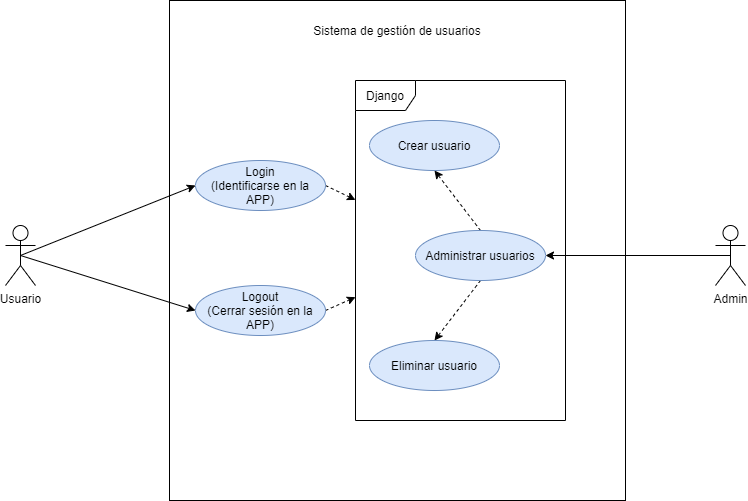
\includegraphics[width=1\textwidth]{imagenes/diagramas_casos_de_uso/CU1-gestion_usuarios.png} 
	\caption{Diagrama de casos de uso referente al sistema de gestión de usuarios de la APP} \label{cu1}
\end{figure}

\subsection{Gestiones de la plataforma de trading (MT5)}

En el diagrama \ref{cu2} se representan los casos de uso referentes a la gestión de la plataforma de trading. Como ya hemos mencionado en los requisitos no funcionales y en otras ocasiones, esta plataforma será \textit{MetaTrader5}. Se mencionará \textit{MetaTrader5} a lo largo del proyecto con la abreviatura \textit{MT5}. \newline

El usuario deberá identificarse con su cuenta, contraseña y servidor en la plataforma en cuestión, MT5. La cuenta podrá ser comercial o demo; y podrá ser creada por cualquier bróker aceptado en MT5. A este caso de uso se le suma el de desconectarse de la cuenta en la que el usuario se ha identificado previamente. \newline

El usuario podrá ver el capital disponible y las operaciones realizadas y en curso. Estos dos casos de uso interactúan internamente con MT5, que es el módulo que nos provee dicha información. La previa identificación del usuario con su cuenta de MT5 será obligatoria para los otros casos de uso.


\begin{figure}[h] 
	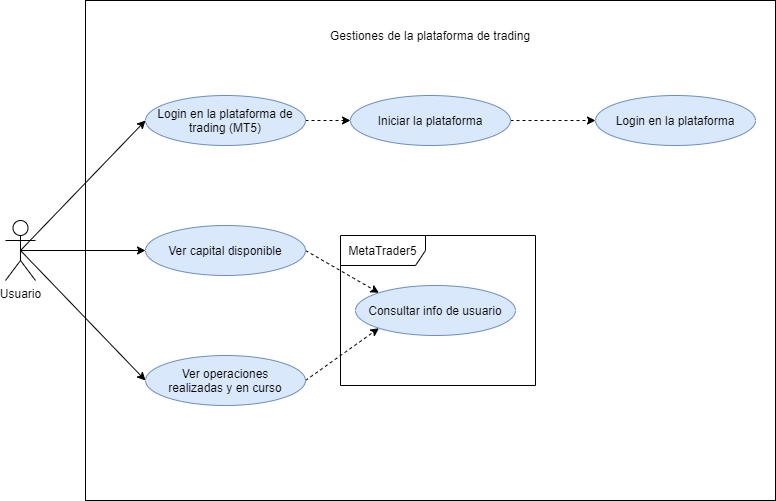
\includegraphics[width=1\textwidth]{imagenes/diagramas_casos_de_uso/CU2-gestiones_MT5.png} 
	\caption{Diagrama de casos de uso referente a la gestión de la plataforma de trading (MT5)}  \label{cu2}
\end{figure}

\subsection{Visualización de datos}

El diagrama \ref{cu3} muestra los casos de uso referentes a la visualización de datos de mercados financieros. Dichos datos serán mostrados mediante un gráfico que muestra precios por medio de velas siguiendo el formato \textit{OHLC}. \newline

El usuario podrá ver datos históricos de mercado en un rango de tiempo específico. Este caso de uso interactúa con los datos proporcionados previamente por el usuario. \newline

El usuario de la APP podrá ver datos en tiempo real con un marco de tiempo específico, es decir, con velas generadas cada minuto, cada hora, cada día, etc. Este \textit{CU} usa el módulo de \textit{MT5} para obtener los datos y luego procesa dichos datos para ajustarlos al formato \textit{OHLC}.


\begin{figure}[h] 
	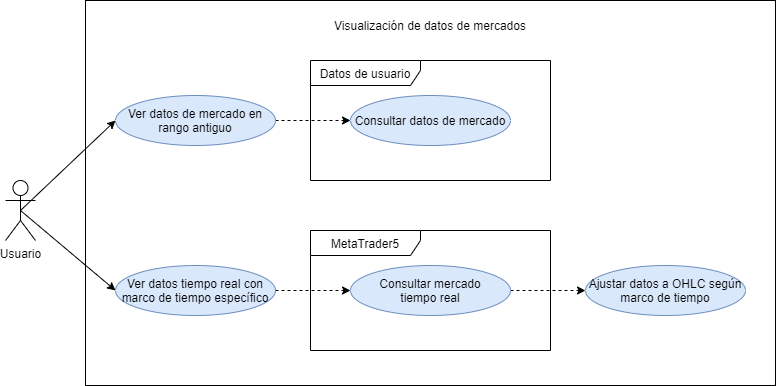
\includegraphics[width=1\textwidth]{imagenes/diagramas_casos_de_uso/CU3-visualizacion_datos.png} 
	\caption{Diagrama de casos de uso referente a la visualización de datos de mercados financieros} \label{cu3}
\end{figure}


\subsection{Funcionalidades de trading}

Finalmente, el diagrama \ref{cu4} representa los casos de uso referentes al módulo de trading y elección de algoritmos. \newline

El usuario podrá elegir un algoritmo de trading. A la hora de operar, el usuario podrá usar el algoritmo elegido para operar en tiempo real o realizar backtesting. El usuario también podrá operar manualmente, siguiendo su propio análisis en tiempo real, sin algoritmo. \newline

Para los casos de uso de operar manualmente o de forma automática en tiempo real, la APP se conectará al módulo de MT5 para ordenar las operaciones de compra o venta.


\begin{figure}[h] 
	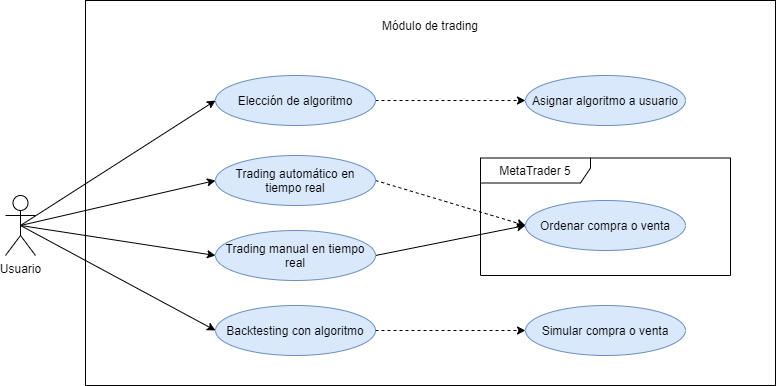
\includegraphics[width=1\textwidth]{imagenes/diagramas_casos_de_uso/CU4-algoritmos.png} 
	\caption{Diagrama de casos de uso referente a las funcionalidades de trading} \label{cu4}
\end{figure}

%

\chapter{Diseño}

% Arquitectura del software, diagramas de clases, diagramas de secuencia

\section{Arquitectura del software}

A continuación muestro un esquema que representa la arquitectura general del software.\newline


\begin{figure}[h]
	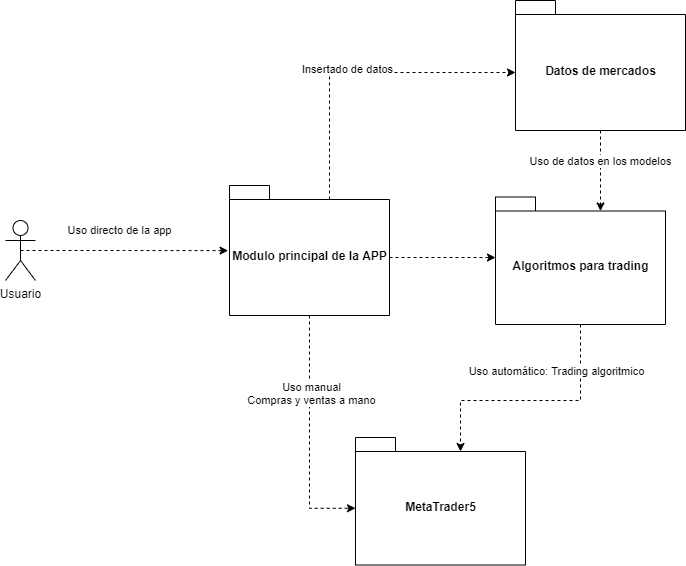
\includegraphics[width=1\textwidth]{imagenes/arquitectura general.png}
	\caption{Arquitectura general del software}
\end{figure}


Como resumen, en el esquema podemos ver cuál es la idea principal del proyecto. El usuario de la aplicación (véase punto \ref{implicados}, segundo implicado) será el que haga un uso directo de la interfaz de la aplicación. A continuación presento cada uno de los módulos con sus funciones y demás utilidades:

\begin{itemize}
	\item \textbf{Módulo principal de la APP}: este módulo se corresponderá con el controlador principal del software. Será usado por el usuario a través de una interfaz escrita en Django y se comunicará con el resto de módulos directamente.
	\item \textbf{Datos de mercados}: este módulo se corresponderá con la base de datos y las operaciones que hagamos con dichos datos (insertado de datos, adaptaciones a cada algoritmo, etc.) Será usado por la interfaz principal de la aplicación y mandará los inputs a los algoritmos.
	\item \textbf{Algoritmos para trading o backend}: se corresponde con el backend o código fuente de la aplicación. Aquí se encontrará cada uno de los algoritmos que usemos para trading algorítmico. Recibe datos de la BBDD y se comunica con el módulo de MetaTrader5 para indicar cada una de las operaciones decididas y obtener información en tiempo real.
	\item \textbf{MetaTrader5}: Módulo externo de la aplicación, se usará para mandar órdenes de operaciones y recibir resultados e información en tiempo real.
\end{itemize}

El software consistirá en una aplicación web con código escrito en Python, usando Django como Framework para la interfaz.

% COMPLETAR CON MAS DETALLES DE HERRAMIENTAS

\section{Primer diseño de la interfaz}

La página web principal mostrará un menú con distintos botones que implementan funcionalidades diferentes. Previo a este menú tendremos un formulario para identificarnos como usuarios de la aplicación. A ambos lados del menú principal y durante todas las vistas de la APP tendremos hiperenlaces con accesos directos a distintas funcionalidades de la aplicación. A continuación muestro una serie de borradores con diseños de cada una de las secciones de la interfaz.\newline

En este primer diseño que muestro en la siguiente imagen, se puede ver el menú principal de la aplicación.\newline

\begin{figure}[h] \label{menu_principal}
	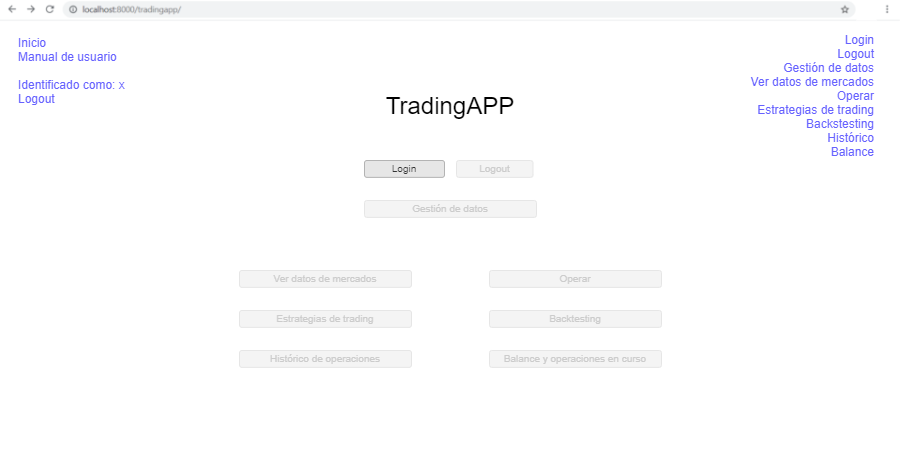
\includegraphics[width=1.2\textwidth]{imagenes/menu_principal}
	\caption{Primer diseño del menú principal de la APP}
\end{figure}

En la imagen mostrada vemos los siguientes botones: \textit{Login}, \textit{Logout}, \textit{Gestión de datos},\textit{ Mi perfil}, \textit{Ver datos de mercados}, \textit{Operar}, \textit{Estrategias de trading}, \textit{Backtesting}, \textit{Histórico de operaciones} y \textit{Balance y operaciones en curso}. En los puntos siguientes explico qué realizaría cada botón y con qué parte del software conectaría.\newline

\begin{itemize}
	\item \textbf{Login}: permite conectar a nuestra cuenta de MetaTrader5, comercial o demo. Véase la siguiente figura. \textit{\textbf{Referencia}: login, RF-1.1.}
	\item \textbf{Logout}: permite cerrar la sesión iniciada anteriormente con el menú de Login. Este botón no estará habilitado hasta que hayamos iniciado sesión. \textit{\textbf{Referencia}: login, RF-1.1.}
	\item \textbf{Gestión de datos}: permite el insertado y procesado de datos de mercado. El usuario podrá a través del menú correspondiente introducir datos al módulo que se encarga de gestionar la BBDD. Al ser un módulo totalmente independiente del módulo de MetaTrader5, no será necesario haber iniciado sesión anteriormente. \textit{\textbf{Referencia}: procesado de datos, RF-2.}
	\item \textbf{Mi perfil}: permite indicar la información del bróker usado. En este menú indicamos información sobre comisiones u otros parámetros.
	\item \textbf{Ver datos de mercados}: permite ver datos de precios de un mercado elegido. Se permite ver datos en un marco de tiempo específico, en rango y de mercados específicos. \textit{\textbf{Referencia}: visualización de datos, RF-3.}
	\item \textbf{Operar}: lleva al usuario a un menú donde podrá operar manualmente, es decir, gestionando las operaciones abiertas y/o abriendo nuevas; o usando el trading algorítmico. \textit{\textbf{Referencia}: operar manualmente, RF-4; trading algorítmico, RF-5.} 
	\item \textbf{Estrategias de trading}: lleva a un menú en el que se puede obtener información de cada una de las estrategias de trading así como elegir una para que sea usada en las próximas operaciones. \textit{\textbf{Referencia}: trading algorítmico, RF-5.} 
	\item \textbf{Backtesting}: menú similar a Operar. En este caso el usuario podrá iniciar operaciones manualmente o usando trading algorítmico a partir de una fecha anterior a la actual, simulando el transcurso del tiempo. \textit{\textbf{Referencia}: backtesting, RF-6.} 
	\item \textbf{Histórico de operaciones}: permite al usuario ver un resumen del histórico de operaciones realizadas. \textit{\textbf{Referencia}: información de operaciones, RF-1.3.} 
	\item \textbf{Balance y operaciones en curso}: permite al usuario ver el capital disponible, así como un balance a tiempo real de pérdidas y ganancias y el resumen de las operaciones en curso. \textit{\textbf{Referencia}: capital disponible, RF-1.2; información de operaciones, RF-1.3.} 
\end{itemize}

A continuación muestro una imagen de lo que sería el menú de \textbf{Login}. En este menú se introducirán Login, Contraseña y Servidor para que nuestra aplicación inicie sesión en la cuenta demo o comercial de MetaTrader5.\newline

\begin{figure}[h]
	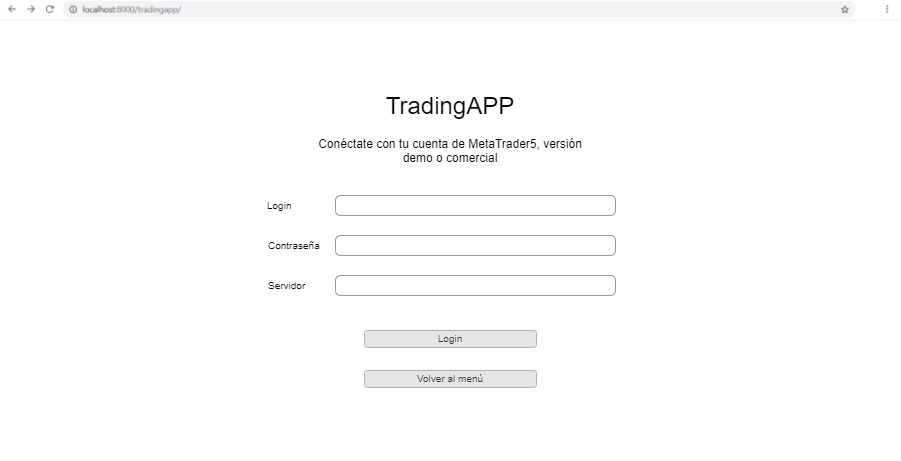
\includegraphics[width=1.2\textwidth]{imagenes/menu_login}
	\caption{Primer diseño del formulario de login en \textit{MT5}}
\end{figure}

Una vez estemos conectados en la cuenta de MT5, nuestro menú principal mostrará disponibles las funcionalidades que en la figura \ref{menu_principal} no estaban habilitadas. Dichas funcionalidades dependen directamente del módulo de MT5, por lo que necesitan de conexión a la cuenta. \newline

\begin{figure}[h]
	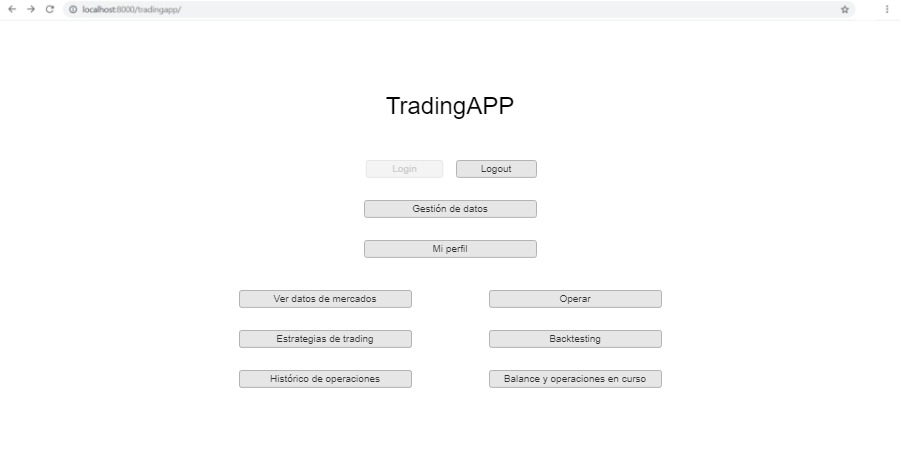
\includegraphics[width=1.2\textwidth]{imagenes/menu_principal_logued}
	\caption{Primer diseño del menú principal (usuario identificado en \textit{MT5}) }
\end{figure}




%



\chapter{Implementación}\label{cap:implementacion}





%
\begin{titlepage}

\chapter{Pruebas}



\end{titlepage}

%
\begin{titlepage}

\chapter{Conclusiones}



\end{titlepage}

%
%%\chapter{Conclusiones y Trabajos Futuros}
%
%
%%\nocite{*}
%\bibliography{bibliografia/bibliografia}\addcontentsline{toc}{chapter}{Bibliografía}
%\bibliographystyle{miunsrturl}
%
%\appendix
%\input{apendices/manual_usuario/manual_usuario}
%%\input{apendices/paper/paper}
%\input{glosario/entradas_glosario}
% \addcontentsline{toc}{chapter}{Glosario}
% \printglossary
\chapter*{}
\thispagestyle{empty}

\end{document}
